\section{Miniboxing Transformation}
\label{sec-mb-traf}

\topic{The miniboxing transformation, which we developed as a Scala compiler plugin, builds upon specialization}, which has been formalized in \cite{iuli-thesis}. It has the same opportunistic and compatible nature and performs class and method duplication in a similar manner. Still, five elements set it apart:

\begin{itemize}
\item the different inheritance scheme (\S\ref{sec-mb-traf-inheritance})
\item the type bytes for storing encoded types (\S\ref{sec-mb-traf-type-bytes}, \S\ref{sec-mb-traf-classes})
\item the use of a shallow type transformation (\S\ref{sec-mb-traf-shallow})
\item the use of the final peephole transformation (\S\ref{sec-mb-traf-peephole})
\item the runtime support for miniboxed values (\S\ref{sec-mb-traf-runtime} and \S\ref{sec-runtime})
\end{itemize}

\begin{figure}[t]
    \centering
    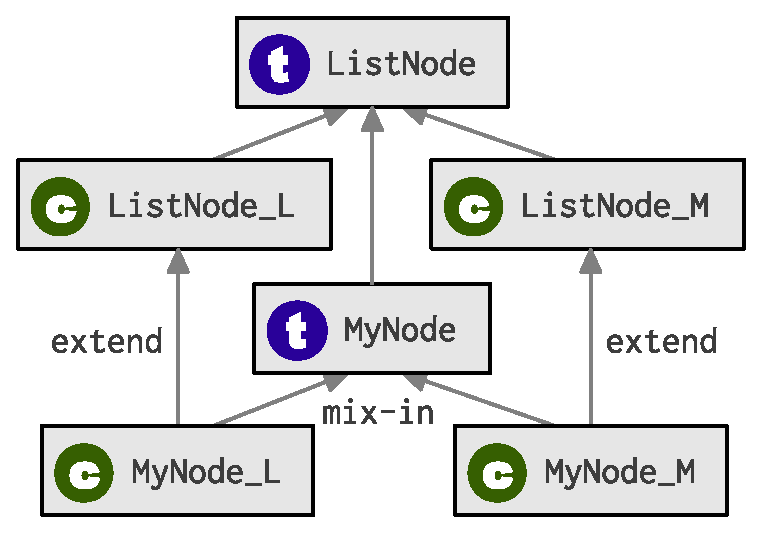
\includegraphics[width=0.30\textwidth]{diags/mbox-multi.eps}
    %\vspace{-18mm}
    \caption{An example of miniboxed class inheritance. The suffixes are: M - miniboxed encoding and L - reference type. Compare to the specialized class inheritance in Figure \ref{fig-spec-multi}.}
    \label{fig-mbox-multi}
\end{figure}


\subsection{Inheritance}
\label{sec-mb-traf-inheritance}
\topic{Miniboxing uses a generic trait as the parent of the specialized classes, therefore} avoiding the limitation that miniboxed classes cannot  inherit from each other (\S\ref{subsec-spec-limits}). Figure \ref{fig-mbox-multi} shows an example miniboxed class inheritance. As explained in \S\ref{subsec-spec-limits}, for $n$ specialized type parameters, having a trait as the parent increases the bytecode size from $2^n$ to $4^n$, since each of the $2^n$ miniboxed variants needs to implement all $2^n$ methods. Still, the extra bytecode is well spent, for two reasons:

\begin{itemize}
 \item Having a trait at the top of the hierarchy means no generic fields are inherited in the specialized variants, as it happens when the homogeneous translation is at the top of the hierarchy (\S\ref{subsec-spec-limits});
 \item This inheritance scheme allows specialized classes to inherit their specialized parent, thus achieving better performance in deep hierarchies.
\end{itemize}

Since the types assigned to tree nodes do not reference the specialized variants but only the generic interface, this inheritance scheme does not interfere with covariance or contravariance. Indeed, if the type parameter of |ListNode| is defined as covariant, |ListNode_M[Int]| is subtype of |ListNode[Int]| and, transitively, of |ListNode[Any]|.

\subsection{Miniboxing Specifics}

This section will work its way from small examples to describing the new elements in the miniboxing transformation, as compared to specialization. In order to simplify the presentation, we will use the |Long|-based encoding for miniboxing, but the transformation can still be generalized to any number of storage types.

\subsubsection{Type Bytes}
\label{sec-mb-traf-type-bytes}

Type-encoding bytes (or type bytes for short) record the original type of the miniboxed values. Translating the following example shows when type bytes are necessary:

\begin{lstlisting-nobreak}
 def print[@minispec T](value: T): Unit = println(value.toString)
\end{lstlisting-nobreak}

Having the type parameter |T| annotated with |@minispec| will trigger miniboxing, which will duplicate this method for |Long|-encoded value types, which we also call miniboxed types. Like specialization, miniboxing produces groups of overloaded methods, with the original method being the all-reference implementation in its group. In our case, only the miniboxed overload needs to be created. To do so, the compiler will create another version of |print| for long integers, which we call |print_M|: 

\begin{lstlisting-nobreak}
 def print_M(value: Long): Unit = println(value.toString)
\end{lstlisting-nobreak}

This is a very naive translation. Calling |print(false)|, after method rewiring, will transform the boolean to a long integer whose value will be printed on the screen instead of the ``false'' string. To perform the correct action, the translation should recover the string representation of the boolean value |false| from the |Long| encoding. This suggests the |toString| operation should be rewritten to: 

\begin{lstlisting-nobreak}
 def print_M(value: Long): Unit = println(MBRuntime.toString(value))
\end{lstlisting-nobreak}

The code above shows a less naive implementation, since it rewires |toString| calls on the miniboxed value to a special runtime support object in order to obtain the string representation. But passing a single miniboxed value isn't enough, as we mentioned miniboxing does not encode the type with the value as tagged unions do \cite{tagged-unions-lua}. Therefore, it should have a separate parameter to encode the original type: 

\begin{lstlisting-nobreak}
 def print_M(T_Type: Byte, value: Long): Unit = println(MBRuntime.toString(value, T_Type))
\end{lstlisting-nobreak}

This is close to the minibox-transformed version of |print_M| the plugin would output. The |T_Type| field only encodes the 9 primitive types in Scala, therefore it does not incur the typical overhead of full reified generics \cite{michel-thesis}. A call to |print(false)| will be translated to the following code, where |BOOLEAN| is the type byte for boolean values:

\begin{lstlisting-nobreak}
 print_M(BOOLEAN, MBRuntime.BoolToMinibox(false))
\end{lstlisting-nobreak}

The method call above shows two differences between rewiring in miniboxing and specialization:
\begin{enumerate}
  \item Calling a miniboxing-transformed method (or instantiating a miniboxing-transformed class) requires passing type bytes for all the |Long|-encoded type arguments;
  \item The arguments to minibox-transformed methods need to be explicitly encoded in the storage type.
\end{enumerate}

We will now present exactly how the miniboxing plugin arrives to this transformed code. As the miniboxing transformation takes place, it needs to preserve program semantics and type correctness. In order to do so, the transformation for |print| is actually done in three steps.

First, the new signature is created, knowing the type parameter |T| is encoded as |Long|. The method name is mangled (mangled names are simplified in this presentation) and the type byte for |T| is added to the signature. Then parameters are added, with all parameters of type |T| being replaced by parameters of type |Long|. As this happens, the symbols whose types changed are recorded and treated specially. In this case, the only miniboxed parameter is |value|, which is recorded. It is also recorded that the type byte |T_Type| corresponds to the encoded type |T|. This yields: (we'll see later why the type parameter |T| still appears)

\begin{lstlisting-nobreak}
 def print_M[T](T_Type: Byte, value: Long): Unit = // need to copy and adapt body from print
\end{lstlisting-nobreak}

In the second step, the body is copied from the |print| method. To maintain type correctness, all the symbols previously recorded as having their types changed are now automatically boxed back to generic type |T|, so the newly generated code tree is consistent in terms of types: 

\begin{lstlisting-nobreak}
 def print_M[T](T_Type: Byte, value: Long): Unit = println(MBRuntime.MiniboxToBox[T](value, T_Type).toString)
\end{lstlisting-nobreak}

In the final step, the tree rewrite rules will transform the call to |MiniboxToBox| followed by |toString| into a single call to the |MBRuntime| system, which typically yields better performance:

\begin{lstlisting-nobreak}
 def print_M[T](T_Type: Byte, value: Long): Unit = println(MBRuntime.toString(value, T_Type))
\end{lstlisting-nobreak}

The next section will explain why it is necessary to carry the type parameter |T|.

\subsubsection{Shallow and Deep Type Transformations}
\label{sec-mb-traf-shallow}
 
To further understand the miniboxing transformation, let us look at a more complex example, which builds a linked list with a single element:

\begin{lstlisting-nobreak}
 def list[@minispec T](value: T): ListNode[T] = new ListNode[T](value, null) 
\end{lstlisting-nobreak}

As explained before, the |list| method will become the all-reference overload. But the interesting transformation happens in the miniboxed variant. If specialization were to transform this method its signature would be:

\begin{lstlisting-nobreak}
 def list_M[T](value: Long): ListNode[Long] 
\end{lstlisting-nobreak}

The return type is incorrect, as we expect |list(3)| to return a |ListNode[Int]|, and yet rewiring |list(3)| to |list_M(...)| would return a |ListNode[Long]|. This exposes the difference between the deep type transformation in specialization and the shallow type transformation in miniboxing: In miniboxing, only values of type |T| are transformed to |Long|, but any type referring to |T|, such as |ListNode[T]|, will remain the same. This explains why the type parameter |T| is carried over to |print_M| and |list_M|: it may still be used in the method's signature and code. The full transformation for method |list_M| will be:

\begin{lstlisting-nobreak}
 def list_M[T](T_Type: Byte, value: Long): ListNode[T] = 
   new ListNode[T](MiniboxToBox[T](value, T_Type))
\end{lstlisting-nobreak}

The shallow type transformation also changes types of local variables from |T| to |Long| and recursively transforms all nested methods and classes within the piece of code it is adapting. This propagates the storage type representation throughout the code.

\subsubsection{Peephole Transformation}
\label{sec-mb-traf-peephole}

The last transformation to touch the code before it is shipped to the next phase is the peephole transformation, which performs a final sweep over the code to remove redundant conversions. To show this phase at work, let us consider what happens if the |ListNode| class in the last example is also annotated for miniboxing. In this case, the class will have a miniboxed variant, |ListNode_M| to which the instantiation is rewired. Since the |head| parameter of the |ListNode| constructor is boxed, while the |head| parameter of the |ListNode_M| constructor is miniboxed, the transformation will introduce a new |BoxToMinibox| conversion:   

\begin{lstlisting-nobreak}
 def list_M[T](T_Type: Byte, value: Long): ListNode[T] = 
   new ListNode_M[T](T_Type, BoxToMinibox[T](MiniboxToBox[T](value, ...)), null)
\end{lstlisting-nobreak}

Converting from |Long| to the boxed representation and back before creating the list node will certainly affect performance. Such consecutive complementary conversions and other suboptimal constructs are automatically removed by the peephole optimization: % After the rewrite, the code for |list_M| will be: 

\begin{lstlisting-nobreak}
 def list_M[T](T_Type: Byte, value: Long): ListNode[T] = 
   new ListNode_M[T](T_Type, value, null)
\end{lstlisting-nobreak}

The code produced by the rewiring phase can be optimized by a single pass of the peephole transformation so there is no need to iterate until a fixed point is reached.

\subsubsection{Type Bytes in Classes}
\label{sec-mb-traf-classes}

The class translation is slightly more complex than method translation. For classes, type bytes are also included as fields in the miniboxed variants, to allow the class' methods to encode and decode miniboxed values as necessary: % An example is the translation for the |ListNode| class:

\begin{lstlisting-nobreak}
 class ListNode[@minispec T]
   (val head: T, val tail: ListNode[T]) {
   def contains(element: T): Boolean = ...
 }
\end{lstlisting-nobreak}

The interface resulting after miniboxing will be:

\begin{lstlisting-nobreak}
 trait ListNode[T] {
   ... // getters for head and tail
   def contains(element: T): Boolean
   def contains_M(T_Type_local: Byte, element: Long): Boolean
 }
\end{lstlisting-nobreak}

And the miniboxed variant of this class will be:

\begin{lstlisting-nobreak}
 class ListNode_M[T]
   (T_Type: Byte, head: Long, tail: ListNode[T]) extends ListNode[T] {
   ... // getters for head and tail
   def contains(element: T): Boolean = 
         ... // redirect to this.contains_M
   def contains_M(T_Type_local: Byte, element: Long): Boolean =
         ... // specialized implementation
 }
\end{lstlisting-nobreak}

|ListNode_M| has two type tags: |T_Type| is a class parameter and becomes a field of the class while |T_Type_local| is passed to the |contains_M| method directly. In the code example, |T_Type| is used to convert the |element| parameter of |contains| to its miniboxed representation when redirecting the call to |contains_M|. But |T_Type_local| is not used in the |ListNode_M| class. To understand when |T_Type_local| is necessary, we have to look at the re\-fe\-rence-carrying variant of the |ListNode| class:

\begin{lstlisting-nobreak}
 class ListNode_L[T]
   (head: T, tail: ListNode[T]) extends ListNode[T] {
   ... // getters for head and tail
   def contains(element: T): Boolean = 
         ... // generic implementation
   def contains_M(T_Type_local: Byte, element: Long): Boolean =
         ... // redirect to this.contains
 }
\end{lstlisting-nobreak}

All instantiations of |ListNode| where the type argument is statically known to be a value type are rewired to |ListNode_M|. The rest of the instantiations are rewired to |ListNode_L|, either because the type argument is not known statically or because it is known to be a reference type. Therefore, there is no reason for |ListNode_L| to carry |T_Type| as a global field. But, in order to allow |contains_M| to decode the miniboxed value |element| into a boxed form and redirect the call |contains|, a local type byte is necessary. Since the |ListNode| interface and its two implementations, |ListNode_L| and |ListNode_M| need to be compatible, the local type byte in |contains_M| is also present for |ListNode_M|, although in the miniboxed class it is redundant. 

\subsection{Calling the Runtime Support}
\label{sec-mb-traf-runtime}

The previous examples have shown how the miniboxing plugin uses the |MBRuntime| object for conversions between unboxed, miniboxed and boxed data representations. But the |MBRuntime| object is not limited to conversions. In Scala, any type parameter is assumed to be a subtype of the |Any| class, so the programmer can invoke methods such as |toString|, |hashCode| and |equals| on generic values. As shown in \S\ref{sec-mb-traf-type-bytes}, these calls can be translated by a conversion to the boxed representation followed by the call, but are further optimized by calling the implementations in |MBRuntime|, which work directly on miniboxed values.  

Aside from conversions and implementations for the methods in the |Any| class, the miniboxing runtime support contains code to allow direct interaction between arrays and miniboxed values. An example that uses arrays is the |ArrayBuffer| class:

\begin{lstlisting-nobreak}
 class ArrayBuffer[@minispec T: Manifest] {
   // fields: 
   private[this] var array = new Array[T](32) 
   ...
   // methods: 
   def getElement(idx: Int): T = array(idx)
   ...
 }
\end{lstlisting-nobreak}

The miniboxed variant |ArrayBuffer_M| is rewritten to call the |MBArray| object to create and access arrays in the miniboxed format: 
  
\begin{lstlisting-nobreak}
 // ArrayBuffer miniboxed variant for primitives:
 class ArrayBuffer_M[T: Manifest](T_Type: Byte) 
                               extends ArrayBuffer[T] {
   // fields:
   private[this] var array: Array[T] = MBArray.mbarray_new(32, T_Type)
   ...
   // methods: 
   def getElement(idx: Int): T = 
       MiniboxToBox(getElement_M(T_Type, idx), ...)
   def getElement_M(T_Type_local: Byte, idx: Int): Long = 
       MBArray.array_get(array, idx, T_Type)
   ...
 }
\end{lstlisting-nobreak}

The implementation of the |MBArray| object is critical to numeric algorithms and performance data structures, as it has to be small enough to be inlined by the just-in-time compiler and structured in ways that return the result as fast as possible for any of the primitive types. The following two sections describe the runtime support for arrays and give technical insights into the pitfalls of the implementation.